\chapter{Evaluación de las variables del modelo}
\label{cap:variables}

Los capítulos anteriores tomaron el modelo actuarial como dado. Este lo somete a
examen: para cada variable --- demográfica, financiera, regulatoria o de
calibración --- se pregunta de dónde viene (imposición normativa, convención
actuarial, estimación estadística o calibración \emph{ad hoc}), cuánto pesa en el
resultado y si afecta la estructura de $\VP$ establecida en el
\cref{cap:estructura} o solo su nivel. El \cref{tab:veredicto} resume la evidencia
disponible; tres componentes que requieren revisión se discuten en la
\cref{sec:variables-debiles}. Esta evaluación no acredita una calibración ni una
validación actuarial independiente del cotizador.

\begin{table}[H]
\centering
\caption[Veredicto sobre las variables del modelo]{Veredicto sobre las variables
del modelo. Las marcadas con \textcolor{rojotesis}{$\bullet$} requieren revisión
y se discuten en detalle en la
\cref{sec:variables-debiles}.}
\label{tab:veredicto}
\small
\begin{tabular}{@{}>{\raggedright\arraybackslash}p{4.6cm}>{\raggedright\arraybackslash}p{3.4cm}>{\raggedright\arraybackslash}p{2.3cm}>{\raggedright\arraybackslash}p{4.0cm}@{}}
\toprule
\textbf{Variable} & \textbf{Fundamento} & \textbf{Efecto} & \textbf{Veredicto} \\
\midrule
Tablas de mortalidad & fuentes por conciliar & alto & \textcolor{naranja}{$\bullet$} trazabilidad pendiente \\
Factores de mejora & convención implementada & $\datoEfectoMejora\%$ & \textcolor{naranja}{$\bullet$} años base por justificar \\
Factor de aplicabilidad & convención de la compañía & medio & \textcolor{naranja}{$\bullet$} magnitud sin validar \\
Independencia entre vidas & hipótesis del modelo & por cuantificar & \textcolor{naranja}{$\bullet$} simplificación demográfica \\
Interés técnico real & supuesto de valoración & $\datoSensTasaAlta\%$ & \textcolor{naranja}{$\bullet$} fuente y fecha por documentar \\
IPC en tres tramos & proyección macro & medio & \textcolor{naranja}{$\bullet$} supuesto por contrastar \\
Deslizamiento & política salarial & bajo & \textcolor{verdetesis}{$\bullet$} determina los racimos \\
SMLV & Decreto 0159/2026 & alto o nulo & \textcolor{verdetesis}{$\bullet$} monto decretado; transitorio \\
Auxilio funerario & Ley 100 & bajo & \textcolor{verdetesis}{$\bullet$} exacta \\
Recargos de gastos & tarifa de la compañía & medio & \textcolor{naranja}{$\bullet$} base por conciliar \\
Sobrecosto de mortalidad RP & tabla de la compañía & medio & \textcolor{naranja}{$\bullet$} sin fuente documentada \\
Beneficiario hipotético & convención de RP & alto & \textcolor{naranja}{$\bullet$} calibración pendiente \\
Curva Smith-Wilson & estándar EIOPA & alto & \textcolor{rojotesis}{$\bullet$} configuración sin validar \\
Volatilidad de la CAI & estimación aproximada & alto & \textcolor{rojotesis}{$\bullet$} sin serie histórica de apoyo \\
Factor de ajuste NI & calibración empírica & alto & \textcolor{rojotesis}{$\bullet$} sin validación independiente \\
\bottomrule
\end{tabular}
\end{table}

\section{Variables demográficas}
\label{sec:var-demograficas}

Las series de mortalidad del archivo de datos están diferenciadas por sexo para
rentistas válidos e inválidos. La Resolución 1555 de 2010 actualiza las tablas de
rentistas válidos RV08 \citep{sfc2010} y la Resolución 0585 de 1994 rige para
invalidez y mortalidad de inválidos \citep{sfc1994}. La denominación de las
columnas de inválidos no basta para atribuirlas a una tabla concreta: su
trazabilidad exige conciliar cada serie con su fuente, población, sexo, año base y
transformaciones. Como control descriptivo, el ajuste de Gompertz
$\ln q_x=\ln A+b\,x$ sobre las edades $40$--$95$ de la serie masculina de
válidos da $b=\datoGompertzB$ ($R^2=\datoGompertzRDos$), es decir, una
duplicación de la mortalidad cada $\datoGompertzDuplica$ años, consistente con el
rango de $7$ a $9$ años de la literatura \citep{pitacco2009}; el ajuste no valida
el nivel de la serie para la cartera.

La implementación aplica mejoras de longevidad $q_x(1-r_x)^{a_t}$, con
$a_t=\min\{30,\,A_t-A_{\mathrm{base}}\}$ y años base $2022$ para válidos y
$1985$ para inválidos, distintos del año que identifica la tabla RV08 y cuyo
origen requiere documentación en la nota técnica;
suprimirlas cambia la reserva de la póliza de referencia en $\datoEfectoMejora\%$.
Multiplica además $q_x$ por $0{,}70$ para el causante válido y por $0{,}95$ para
los beneficiarios válidos. La selección de rentistas puede motivar ajustes de
experiencia, pero la información disponible no aporta un estudio que justifique
estos valores.
Una reducción del $30\%$ en la mortalidad es considerable y, cuando la tabla de
partida ya representa rentistas, debe verificarse que el ajuste no duplique un
efecto de selección incorporado previamente; su calificación adecuada es
«defendible en concepto, no verificada en magnitud».

\label{sec:var-dependencia}%
La \cref{prop:conab} supone independencia entre vidas, aunque la literatura
documenta dependencia en la mortalidad conyugal \citep{frees1996}; su efecto sobre
la reserva no se cuantifica aquí. Si solo se modifica $\CONAB(t)$, independiente
de $M$, cambian los pesos $w_t$ de \cref{eq:canonica} pero se conservan la
representación afín a trozos y el conjunto de umbrales candidatos; las propiedades
que exigen pesos positivos deben verificarse de nuevo.

Sobre la póliza de referencia, la variable demográfica dominante es la presencia de
cónyuge beneficiaria: suprimirla cambia la reserva en $\datoEfectoConyuge\%$,
al retirar la cobertura de sobrevivencia de esa beneficiaria y pasar de dos vidas
a una. El régimen de catorce mesadas la cambia en $\datoEfectoCatorce\%$, cerca
de $1/13$, y un causante inválido en $\datoEfectoInvalido\%$.

\section{Variables financieras y regulatorias}
\label{sec:sensibilidad}

En la póliza de referencia, la tasa de interés técnico tiene un efecto relevante:
una variación de $\pm50$ puntos básicos mueve la mesada en
$\datoSensTasaAlta\%$ / $\datoSensTasaBaja\%$. Esa sensibilidad es específica del
escenario y debe distinguirse del error de resolución numérica; la
elección de la tasa requiere una justificación actuarial independiente de la
rapidez del solucionador. El esquema de inflación en tres tramos
($\datoIPCuno\%$, $\datoIPCdos\%$, $\datoIPClp\%$) es un supuesto de proyección
del cotizador. La indexación de pagos y su incorporación al descuento pueden
compensarse parcialmente; la magnitud depende de las convenciones monetarias y
no debe interpretarse como una cancelación general ni como validación de esa
proyección.

El deslizamiento $\delta=\datoDeslizamiento\%$ tiene un efecto pequeño en el
nivel de la reserva del caso examinado, pero un papel estructural: separa los
umbrales de distintos años.
Con $\delta=0$ los tres racimos colapsan en tres quiebres aislados; un
deslizamiento agresivo los ensancharía hasta solaparlos y destruiría la región afín
comercial. La razón geométrica $\rho=\datoRhoQuiebre$ resume esa dependencia.

El escenario con fecha de valoración del 31 de julio de 2026 utiliza
$S_0=\$\,\datoSMLV$, monto fijado transitoriamente en el artículo 1 del Decreto
0159 de 2026 \citep{presidencia2026smlv}. Su artículo 2 condiciona la vigencia al
fallo del proceso de nulidad allí identificado; aplicar el parámetro a otra fecha
requiere conciliar esa vigencia. El auxilio funerario y el régimen de mesadas
incorporan reglas legales cuya aplicación depende de las condiciones de cada
póliza. El auxilio es, además, el responsable de la pérdida de convexidad del
\cref{thm:no-convexidad}. La sensibilidad al salario mínimo depende de la región:
en el tramo comercial es pequeña, aunque no nula, y en el escenario A-R2 un
aumento del $5\%$ deja el capital por debajo del mínimo financiable, un caso de
capital insuficiente y no una variación de mesada sobre una raíz válida.
En A-R2 también resulta insuficiente el capital al reducir la tasa técnica
en 50 puntos básicos. En ambos casos se omite el porcentaje de cambio de
mesada y se registra el estado de financiación.

En retiro programado, el recargo de mortalidad por edad y sexo (entre el $3{,}8\%$
y el $18\%$) y el cónyuge hipotético que se crea cuando no hay beneficiarios
declarados son convenciones del cotizador. Su fundamento, población objetivo y
calibración no están documentados en las fuentes disponibles; su eventual
justificación prudencial requiere evidencia propia.

\section{Tres componentes que requieren revisión}
\label{sec:variables-debiles}

\subsection{La curva Smith-Wilson}

El modelo de Smith-Wilson \citep{smith2001,eiopa2019}, estándar europeo bajo
Solvencia~II para extrapolar la curva de descuento hacia una tasa forward última
(UFR), está implementado en el motor (\cref{fig:descuento}(b)) pero
\emph{desactivado} en la configuración de referencia. Se
usa con \emph{un solo punto observado} --- el interés técnico del año $1$ --- y
una UFR del $\datoUFR\%$ muy inferior a él, con $\alpha=\datoAlphaSW$ sin
calibrar. Un único nodo no identifica una estructura de mercado entre plazos.
La magnitud de la reserva resultante no valida ni refuta por sí sola el método;
se requiere una calibración documentada con observaciones suficientes y bases
monetarias coherentes, y un contraste frente a curvas alternativas.

\subsection{La volatilidad de la cuenta individual}

El rendimiento anual de la cuenta individual se simula como una normal de media
$\datoCrecCAI\%$ y desviación $\datoVolCAI\%$. La propia documentación del código
reconoce que la desviación es una \emph{estimación} construida con dos
observaciones publicadas y la composición del portafolio, no con la serie
histórica de rentabilidad. La trayectoria proyectada del retiro programado depende
de este parámetro. Su estimación debe apoyarse en una serie histórica con
frecuencia, ventana y base monetaria explícitas y evaluar la adecuación de la
hipótesis normal. Una $t$ de Student escalada permite explorar colas más pesadas,
pero sigue siendo simétrica; el remuestreo por bloques es otra alternativa que
debe contrastarse, sin atribuirle una mejora automática.

\subsection{El factor de ajuste NI}

El modelo dispone de un multiplicador de referencia de $\datoFactorNI$ sobre la
reserva de retiro programado, que se activa cuando la mesada de renta vitalicia
concuerda con una columna de la base dentro de una tolerancia relativa del $5\%$.
La documentación describe una calibración inicial sobre cuatro casos, con factores
entre $1{,}153$ y $1{,}233$, y la implementación admite además una calibración por
póliza que fija el factor como el cociente entre el capital y la reserva evaluada
en la mesada de referencia.

\begin{criticism}[Calibración y validación del factor]
\label{crit:factor-ni}
El procedimiento presenta tres limitaciones. Cuatro
observaciones, con un rango del $7\%$, no acreditan estabilidad ni generalización
del multiplicador. No se propone ninguna interpretación actuarial del factor, de
modo que su uso es una corrección empírica cuya transferencia a otros casos
requiere validación. Y hay circularidad: el criterio de activación usa una
referencia de la base y la calibración por póliza puede imponer la reproducción de
esa misma referencia, así que la concordancia obtenida no acredita desempeño
predictivo. La discrepancia que el factor corrige --- entre el $15\%$ y el
$23\%$ --- es demasiado grande para ser un residuo de redondeo y requiere una
conciliación de componentes. Su uso como corrección transferible requiere
identificar su origen actuarial y separar los casos de calibración de los de
evaluación.
\end{criticism}

A estas variables se suman cuatro ajustes discrecionales del retiro programado:
un piso de crecimiento mínimo, un techo comercial que fuerza que la renta
vitalicia supere al retiro programado (opcional, y desactivado en la
parametrización por defecto), un arranque del primer año igual a la renta
vitalicia y un límite del $50\%$ a la caída anual. Son reglas de la
implementación, distintas de las obligaciones normativas y de la mesada obtenida
por equivalencia actuarial. El arranque $\mathrm{RP}=\mathrm{RV}$ es una regla
de inicialización; los otros ajustes actúan en la recursión. La trayectoria pagada
combina hasta cuatro reglas (tres con la parametrización por defecto), y exige
identificar cuál determina el pago y cómo depende de la mesada anterior
(\cref{cap:retiro}). La forma afín a trozos se refiere a las funciones de ajuste
con referencias fijas, no a una afirmación de linealidad de toda la trayectoria.

\section{Contraste con cotizaciones de referencia}
\label{sec:validacion}

Se comparan las mesadas calculadas con las reportadas para siete pólizas
(\cref{fig:validacion}). La discrepancia media es de $\datoValidMedia\%$, con
extremos de $\datoValidMin\%$ y $\datoValidMax\%$, y en estos casos las mesadas
calculadas son mayores que las de referencia. La causa no está identificada con la
información disponible: deben conciliarse fechas, capitales, tablas, tasas, gastos
y convenciones de pago, y la diferencia no se atribuye a un factor actuarial
omitido sin evidencia adicional. El contraste evalúa concordancia de resultados,
no valida por separado los parámetros del modelo, y su aceptación requiere fijar
una tolerancia de materialidad.

\begin{figure}[H]
\centering
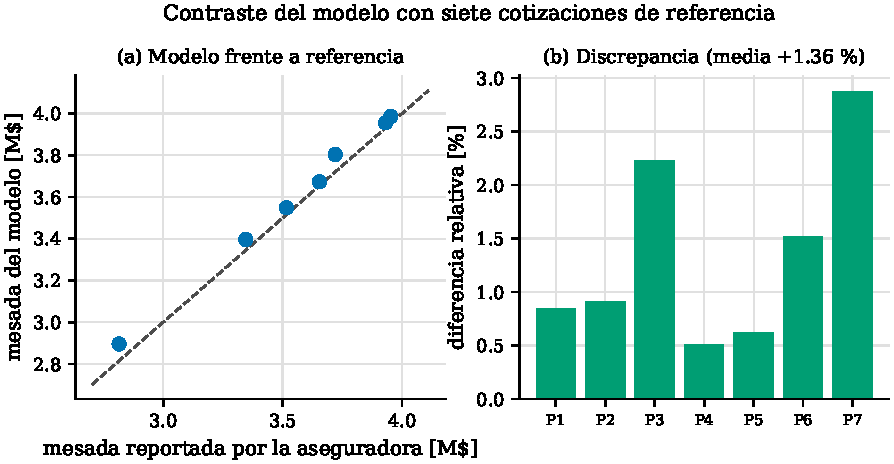
\includegraphics[width=\textwidth]{figuras/fig_validacion}
\caption[Contraste con cotizaciones reales]{Comparación del modelo con las
cotizaciones de referencia de la compañía para siete pólizas. La discrepancia media es de
$\datoValidMedia\%$, con un máximo de $\datoValidMax\%$.}
\label{fig:validacion}
\end{figure}

\section{Síntesis}

La revisión distingue datos normativos, hipótesis de valoración y convenciones del
cotizador. La procedencia de las series de mortalidad, los años base de mejora y
los ajustes de aplicabilidad requieren conciliación documental, y la volatilidad
de la cuenta individual, la calibración de Smith-Wilson y el factor NI limitan la
interpretación actuarial de las proyecciones. Para el análisis numérico, lo
esencial es que las modificaciones que solo alteran pesos independientes de $M$
conservan la representación afín a trozos de \cref{eq:canonica}; la posición de la
raíz y el desempeño de los métodos sí pueden cambiar, y la conservación de la forma
funcional no sustituye la validación de las bases actuariales.
